\documentclass{beamer}

\usetheme{CambridgeUS}
\usecolortheme{orchid}

\usepackage{wrapfig}
\usepackage{siunitx}
\usepackage{inconsolata}
\usepackage{amsmath}
\usepackage{bm}
\usepackage{nicefrac}
\usepackage{tikz}
\usetikzlibrary{shapes.geometric, positioning}

% Approximately equal to
\newcommand{\appropto}{\mathrel{\vcenter{
      \offinterlineskip\halign{\hfil$##$\cr
        \propto\cr\noalign{\kern2pt}\sim\cr\noalign{\kern-2pt}}}}}

% Smiley and frowney items
\newcommand{\startsmitemize}{\vspace{0.15cm}}
\newcommand{\smitem}{\vspace{0.1cm}\noindent\smiley\;}
\newcommand{\fritem}{\vspace{0.1cm}\noindent\frownie\;}

% Number systems, fields, rings, groups...
\newcommand{\bbR}{\mathbb{R}}
\newcommand{\bbC}{\mathbb{C}}
\newcommand{\bbZ}{\mathbb{Z}} 
\newcommand{\bbN}{\mathbb{N}}
\newcommand{\bbS}{\mathbb{S}}

% Calligraphic style
\newcommand{\cA}{\mathcal{A}}
\newcommand{\cB}{\mathcal{B}}
\newcommand{\cD}{\mathcal{D}}
\newcommand{\cE}{\mathcal{E}}
\newcommand{\cF}{\mathcal{F}}
\newcommand{\cI}{\mathcal{I}}
\newcommand{\cL}{\mathcal{L}}
\newcommand{\cM}{\mathcal{M}}
\newcommand{\cN}{\mathcal{N}}
\newcommand{\cO}{\mathcal{O}}
\newcommand{\cP}{\mathcal{P}}
\newcommand{\cS}{\mathcal{S}}
\newcommand{\cT}{\mathcal{T}}

% Roman style
\newcommand{\rmK}{\mathsf{K}}
\newcommand{\rmM}{\mathsf{M}}
\newcommand{\rmP}{\mathsf{P}}
\newcommand{\rmS}{\mathsf{S}}

\newcommand{\rmm}{\mathsf{m}}
\newcommand{\rmp}{\mathsf{p}}
\newcommand{\rms}{\mathsf{s}}

\newcommand{\rmsp}{\mathsf{sp}}

% Symbols
\newcommand{\defeq}{\vcentcolon=}
\newcommand{\eqdef}{=\vcentcolon}

% Symbols in special fonts
\newcommand{\blfa}{{\sf a}}
\newcommand{\lfl}{{\ell}}
\newcommand{\ii}{\mathsf{i}}
\newcommand{\ee}{\mathsf{e}}

% Algorithmic
\newcommand{\BREAK}{\STATE \textbf{BREAK}}

\usefont{T1}{cmtt}{m}{n}

% Notes, etc.
\newcommand{\todo}[1]{{\color{red}\textbf{TODO:} #1}}

% Operators
\DeclareMathOperator{\lcm}{lcm}
\DeclareMathOperator{\supp}{supp}
\DeclareMathOperator{\idty}{Id}
\DeclareMathOperator{\spann}{span}
\DeclareMathOperator{\Mod}{mod}

\newcommand{\dd}{\,\text{d}}
\newcommand{\fdd}{\text{d}}

% Shearlet chapter notation
\newcommand{\aPsi}[5]{\Psi_{#1,#2,#3}^{#4,#5}}
\newcommand{\numatlevel}{\operatorname{NumAtLevel}}
\newcommand{\numright}{\operatorname{NumRight}}
\newcommand{\numup}{\operatorname{NumUp}}
\newcommand{\numshears}{\operatorname{NumShears}}
\newcommand{\nummothers}{\operatorname{NumMothers}}
\newcommand{\stepright}{\operatorname{StepRight}}
\newcommand{\stepup}{\operatorname{StepUp}}
\newcommand{\shear}{\operatorname{Shear}}
\newcommand{\basetrf}{\operatorname{BaseTransform}}
\newcommand{\trf}{\operatorname{Transform}}
\newcommand{\corners}{\operatorname{Corners}}
\newcommand{\checkintersection}{\operatorname{CheckIntersection}}
\newcommand{\computeintersection}{\operatorname{ComputeIntersection}}
\newcommand{\splitpolygon}{\operatorname{SplitPolygon}}
\newcommand{\transformquadrule}{\operatorname{TransformQuadrule}}
\newcommand{\builddquadrule}{\operatorname{BuildDoubleQuadrule}}
\newcommand{\buildsquadrule}{\operatorname{BuildSingleQuadrule}}
\newcommand{\evalblf}{\operatorname{EvalBLF}}
\newcommand{\evallf}{\operatorname{EvalLF}}
\newcommand{\preparepoints}{\operatorname{PreparePoints}}
\newcommand{\modd}{\;\operatorname{\textbf{mod}}\;}

% Boltzmann chapter notation
\newcommand{\Bt}{\tilde{B}}
\newcommand{\B}{\mathcal{B}}
\newcommand{\Bsr}{\B_{\sqrt{2}R}}
\newcommand{\Btr}{\B_{2R}}
\newcommand{\AFF}{\cA_\text{FF}}
\newcommand{\ml}{\lambda^{(+)}}
\newcommand{\LtDl}{{L^2(\cD_L)}}
\newcommand{\PA}{{P_\cA}}
\newcommand{\Qt}{Q_\text{lin}}

% Circled characters
\newcommand*\circled[1]{\tikz[baseline=(char.base)]{
    \node[shape=circle,draw,inner sep=2pt] (char) {#1};}}


\begin{document}

\title[Mixed-order poroelasticity]{A mixed-order isogeometry solver for poroelasticity problems}
\author[E. Fonn]{
  E.~Fonn\inst{1,2} \and
  Y.~W.~Bekele\inst{3} \and
  T.~Kvamsdal\inst{4} \and
  A.~M.~Kvarving\inst{2} \and
  S.~Nordal\inst{3}
}
\institute[SINTEF]{
  \inst{1}%
  \url{eivind.fonn@sintef.no}
  \and \inst{2}%
  Applied Mathematics, SINTEF ICT
  \and \inst{3}%
  Department of Civil and Transport Engineering, NTNU
  \and \inst{4}%
  Department of Mathematical Sciences, NTNU
}
\date[IGA 2015]{}

\titlegraphic{\includegraphics[width=0.3\textwidth]{common/sintef}}

\begin{frame}
  \titlepage{}
\end{frame}

\begin{frame}
  \frametitle{Overview}

  Essentially\ldots
  \begin{enumerate}
  \item Equations
  \item Pictures
  \end{enumerate}
\end{frame}

\section{Poroelasticity}

\begin{frame}
  \frametitle{Poroelasticity}

  Models flow and deformation in porous media by coupling (linear) elasticity
  with Darcy flow. \\~\\
  
  The equilibrium equation:
  \[
    \nabla \underbrace{\left(\bm{\sigma}' - \alpha p \bm{I} \right)}_{\text{total stress}} + \bm{F} = 0
  \]
  We use a linear stress-strain relationship with small displacements.
  \[
    \bm{\sigma}' = \bm{D} :
    \underbrace{\frac{1}{2}\left( \nabla \bm{u} + \nabla \bm{u}^\intercal \right)}_{\text{strain}}
  \]
\end{frame}

\begin{frame}
  \frametitle{Poroelasticity}

  Change of fluid content:
  \[
    \frac{\fdd}{\fdd t}\left( \frac{p}{M} + \alpha \nabla \cdot \bm{u} \right) =
    - \nabla \cdot \bm{v}_f + s
  \]
  Darcy's law:
  \[
    \bm{v}_f = -\bm{\kappa}(\nabla p - \rho_f \bm{g})
  \]
  Here, $\alpha$ is \emph{Biot's coefficient} and $\nicefrac{1}{M}$ is the
  \emph{constrained specific storage coefficient}.
\end{frame}

\begin{frame}
  \frametitle{Poroelasticity}

  The model in final form (and Voigt notation):
  \begin{align*}
    \bm{L}^\intercal \bm{CLu} - \alpha \bm{L}^\intercal \bm{m} p + \bm{F} &= 0 \\
    \alpha \nabla \cdot \dot{\bm{u}} + \frac{1}{M}\dot{p}
    - \nabla \cdot \bm{\kappa}(\nabla p - \rho_f\bm{g}) - s &= 0
  \end{align*}
  Here, $\bm{m}$ and $\bm{L}$ are the Voigt notation identity matrix and
  differential operator.
  \[
    \bm{m} = \begin{pmatrix} 1 \\ 1 \\ 1 \\ 0 \\ 0 \\ 0 \end{pmatrix} \qquad
    \bm{L} = \begin{pmatrix}
      \partial_x & & \\
      & \partial_y & \\
      & & \partial_z \\
      & \partial_z & \partial_y \\
      \partial_z & & \partial_x \\
      \partial_y & \partial_x &
    \end{pmatrix}
  \]
\end{frame}

\section{Finite element discretization}

\begin{frame}
  \frametitle{Finite element discretization}

  \[
    \begin{pmatrix} & \\ \bm{Q}^\intercal & \bm{S} \end{pmatrix}
    \begin{pmatrix} \dot{\bm{u}} \\ \dot{\bm{p}} \end{pmatrix} +
    \begin{pmatrix} \bm{K} & -\bm{Q} \\ & \bm{H} \end{pmatrix}
    \begin{pmatrix} \bm{u} \\ \bm{p} \end{pmatrix} =
    \begin{pmatrix} \bm{f}_u \\ \bm{f}_p \end{pmatrix}
  \]
  Where
  \begin{align*}
    \bm{K} &= \int_\Omega \bm{B}^\intercal \bm{CB} \qquad
             & \bm{B} &= \bm{L} \bm{N}_u \\
    \bm{Q} &= \int_\Omega \bm{B}^\intercal \alpha \bm{m} \bm{N}_u \qquad
             & \bm{f}_u &= \int_\Omega \bm{N}_u^\intercal \bm{F}
                          + \int_{\Gamma_t} \bm{N}_u^\intercal \bm{t} \\
    \bm{H} &= \int_\Omega \nabla \bm{N}_p^\intercal \bm{\kappa} \nabla \bm{N}_p \qquad
             & \bm{f}_p &= \int_\Omega \nabla \bm{N}_p^\intercal \bm{\kappa} \rho_f \bm{g}
                          + \int_\Omega \bm{N}_p^\intercal s
                          - \int_{\Gamma_q} \bm{N}_p^\intercal \bm{q} \\
    \bm{S} &= \int_\Omega \bm{N}_p^\intercal \frac{1}{M} \bm{N}_p
  \end{align*}
\end{frame}

\begin{frame}
  \frametitle{Symmetrized FE discretization}

  We can time-differentiate the equilibrium equation to obtain a symmetric system.
  \[
    \begin{pmatrix} -\bm{K} & \bm{Q} \\ \bm{Q}^\intercal & \bm{S} \end{pmatrix}
    \begin{pmatrix} \dot{\bm{u}} \\ \dot{\bm{p}} \end{pmatrix} +
    \begin{pmatrix} & \\ & \bm{H} \end{pmatrix}
    \begin{pmatrix} \bm{u} \\ \bm{p} \end{pmatrix} =
    \begin{pmatrix} -\dot{\bm{f}_u} \\ \bm{f}_p \end{pmatrix}
  \]
  For the following experiments, we use the backwards Euler time-stepping
  scheme. \\~\\

\end{frame}

\section{Implementation}

\begin{frame}
  \frametitle{Implementation}

  The implementation was done in IFEM, which was presented on Monday by
  A.~M.~Kvarving. Basis functions are B-splines, typically up to
  \textbf{quartics} for the displacement and \textbf{cubics} for the pressure.
\end{frame}

\section{Novelty}

\begin{frame}
  \frametitle{Pressure oscillations}

  Traction is applied instantaneously, but the excess pore pressure can take a
  long time to dissipate. In cases with low permeability, this can cause boundary
  layers with rapidly changing pressure, leading to spurious oscillations. \\~\\

  We hope to alleviate this problem using a mixed-order method, where
  displacements have order $n$ and pressure order $n-1$. \\~\\

  Note: This is \emph{not} a div-compatible formulation, which is expected to
  help even more. 
\end{frame}

\section{1D Consolidation}

\begin{frame}
  \frametitle{1D Consolidation}

  \begin{center}
    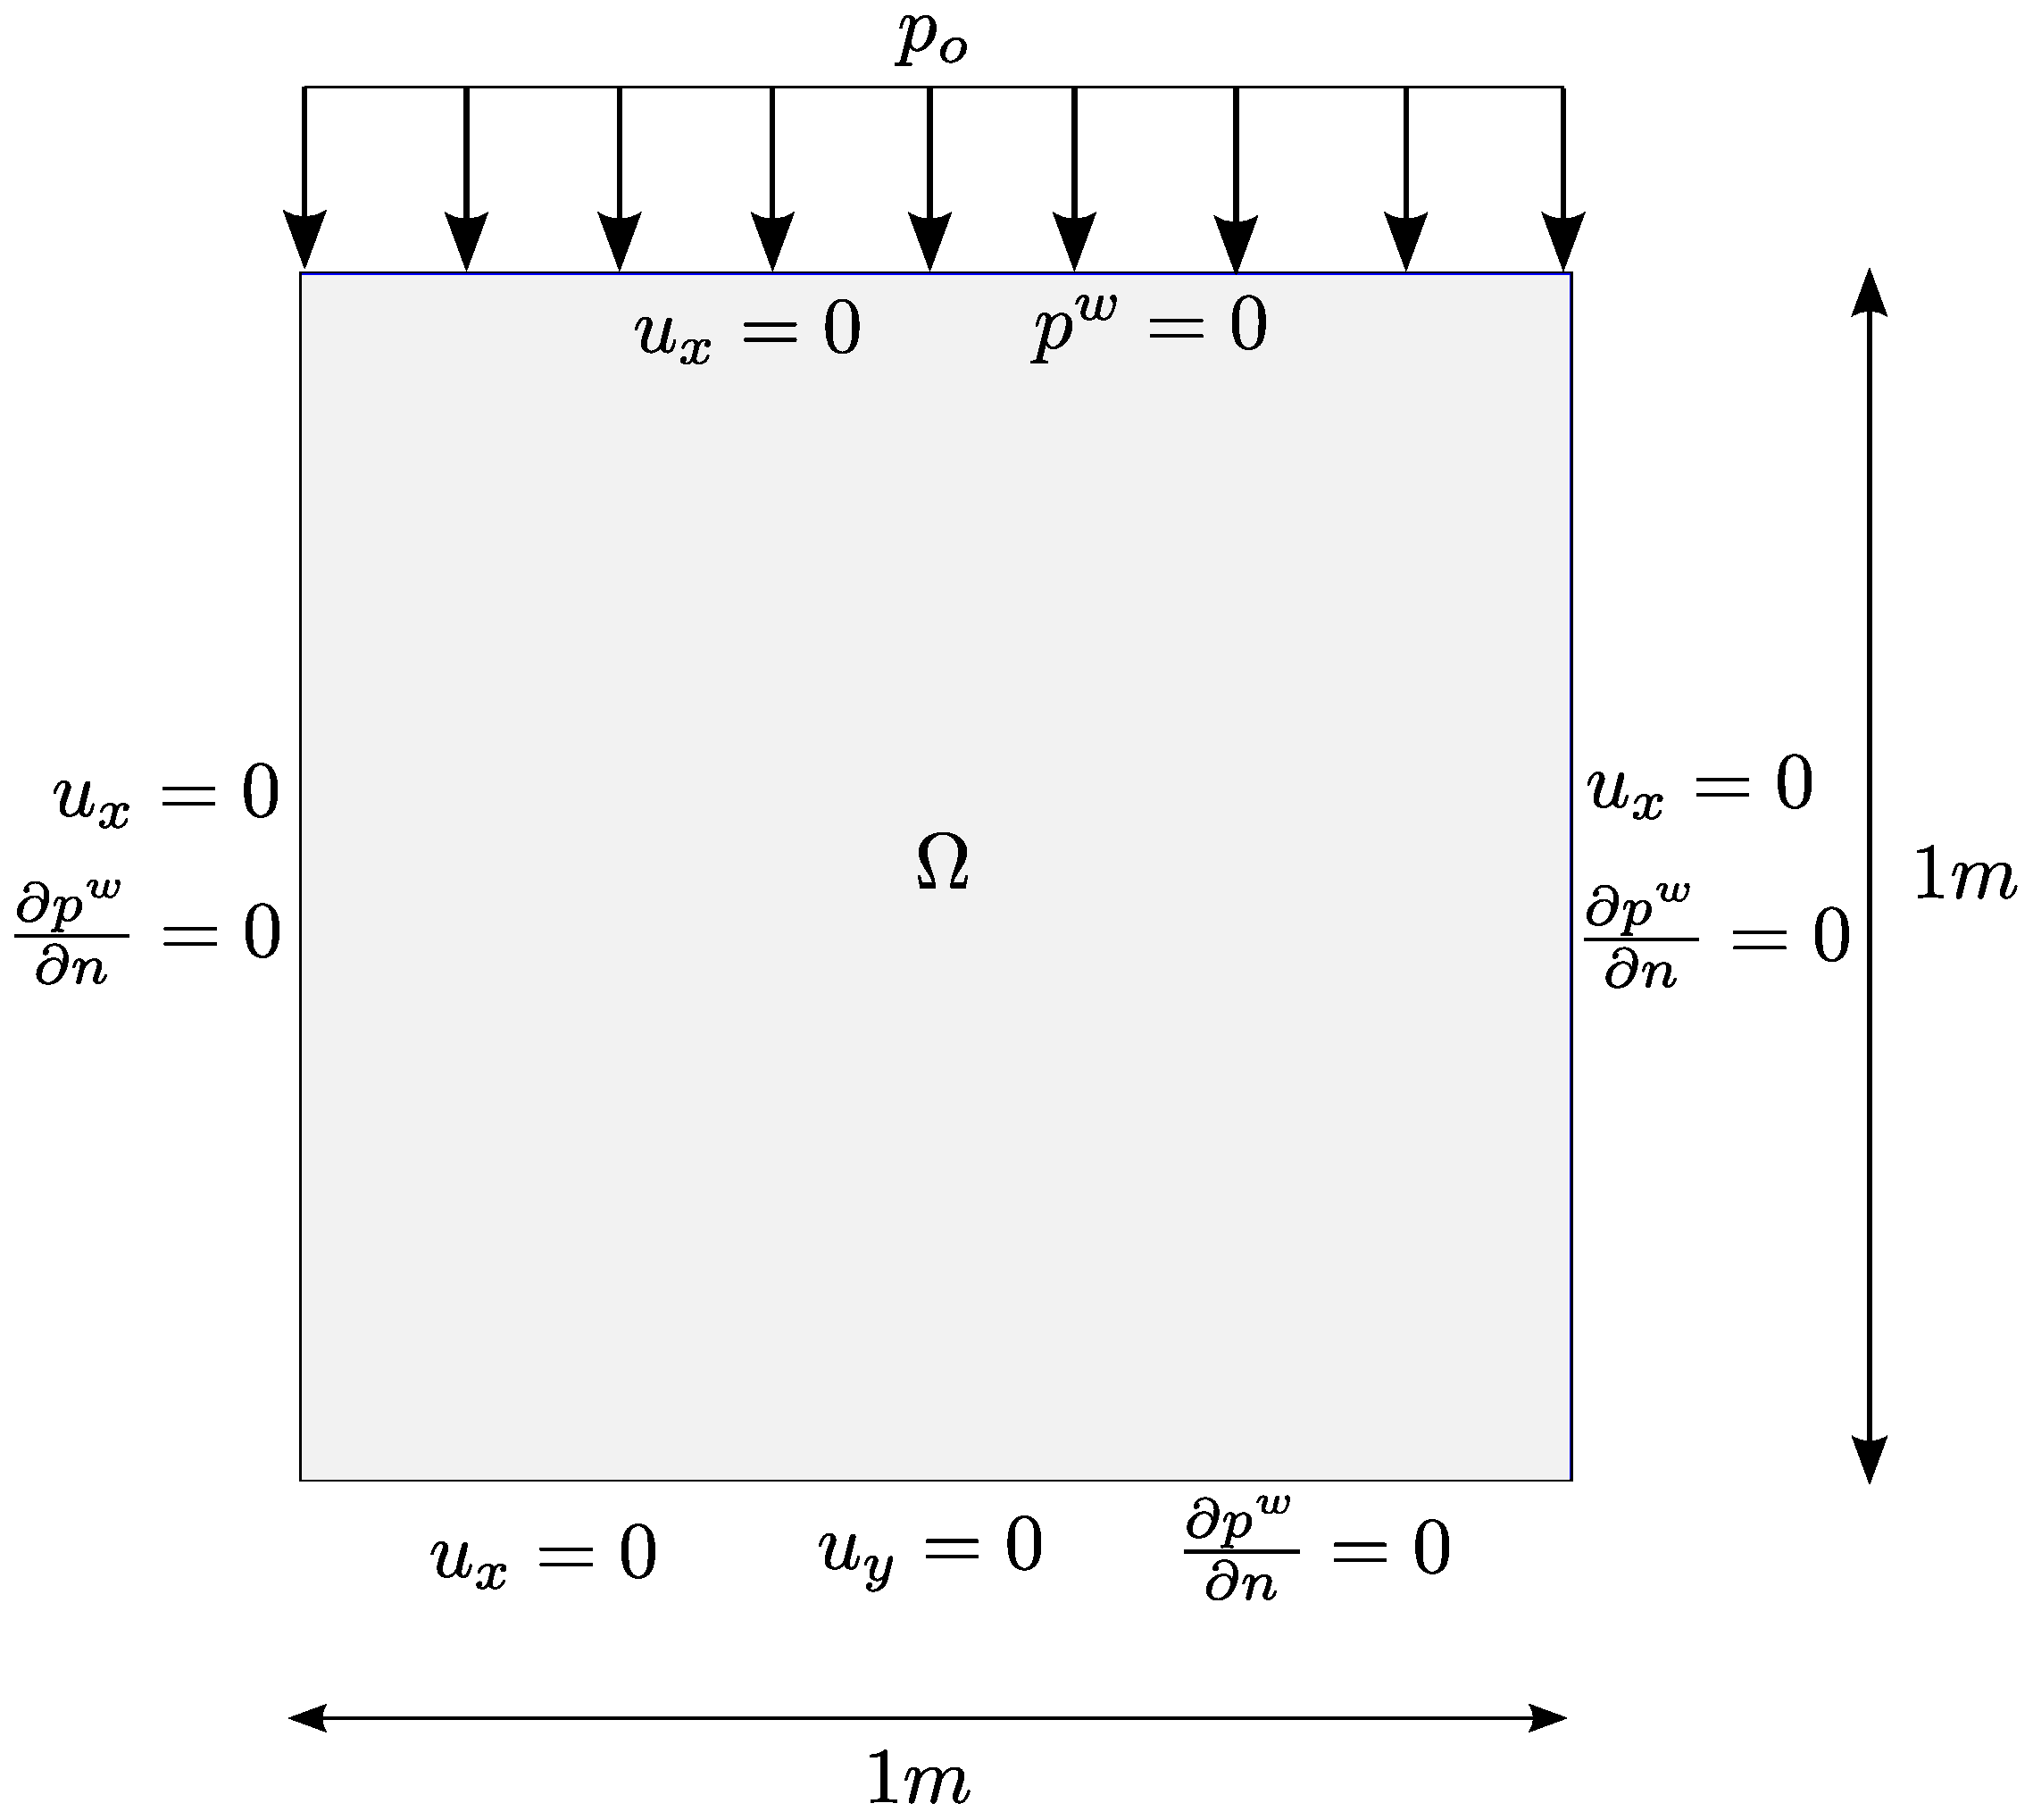
\includegraphics[height=7cm]{figs/Benchmark1}
  \end{center}
\end{frame}

\begin{frame}
  \frametitle{1D consolidation}

  \begin{align*}
    E &= \SI{1}{\mega\pascal} \qquad & \nu &= 0 \\
    k &= \SI{11.57}{\nano\meter\per\second} \qquad & p_0 &= \SI{1}{\mega\pascal}
  \end{align*}

  Analytical solution:
  \[
    \frac{p}{p_0} = \frac{4}{\pi}
    \sum_{i=1}^\infty \frac{(-1)^{i-1}}{2i-1}
    \cos\left[ (2i-1) \frac{\pi y}{2 h} \right]
    \exp\left[ -(2i-1)^2 \frac{\pi^2 c_v t}{4h^2} \right]
  \]
  where $c_v$ is the consolidation coefficient
  \[
    c_v = \kappa \left( \frac{1}{M} + \frac{\alpha^2}{K + \frac{4}{3}G} \right)^{-1}
  \]
\end{frame}

\begin{frame}
  \frametitle{1D consolidation}

  \begin{center}
    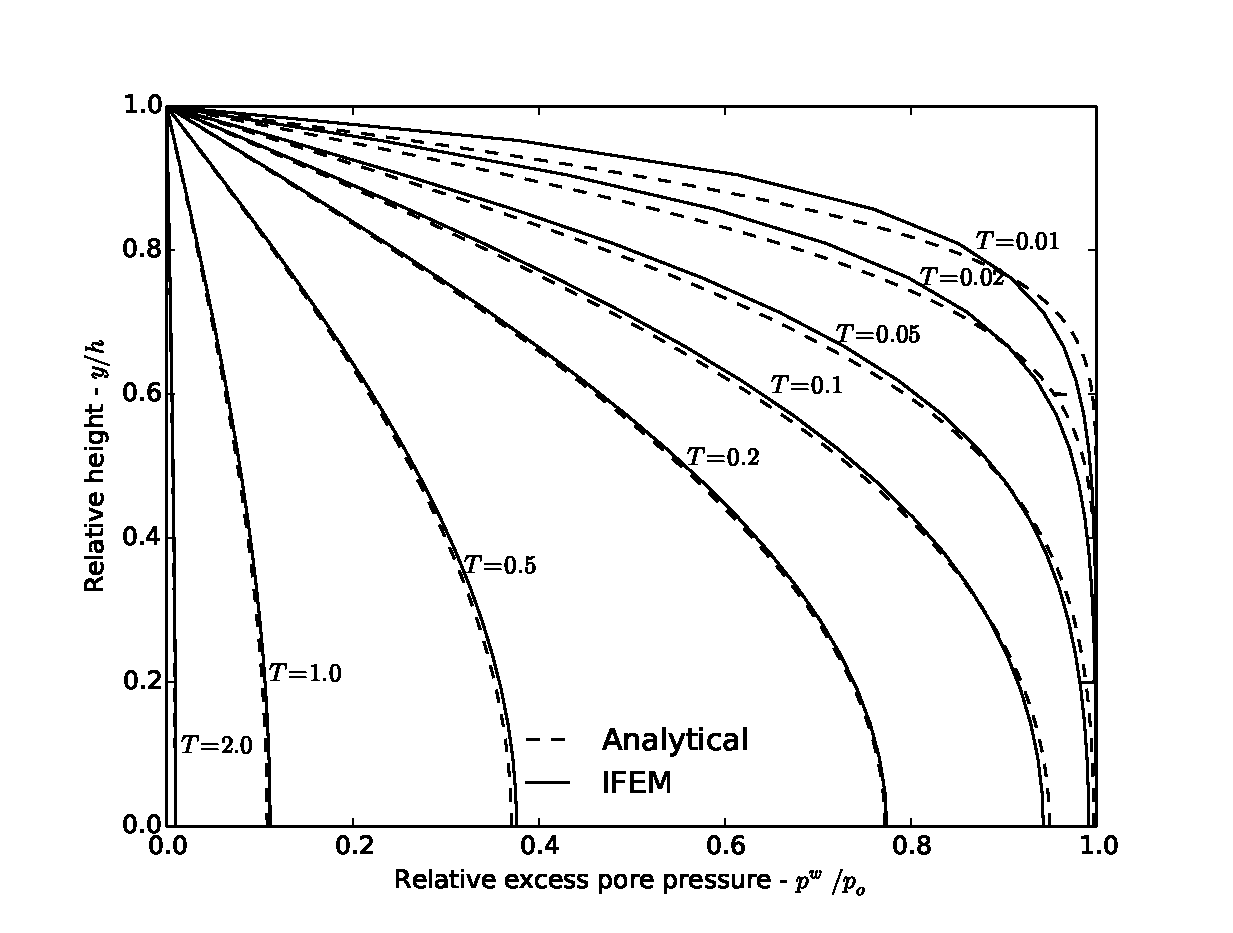
\includegraphics[height=7cm]{figs/PLAXIS_Anasol_v_IFEM}
  \end{center}
\end{frame}

\begin{frame}
  \frametitle{1D consolidation}

  \vspace{-3.5cm}
  \begin{wrapfigure}{l}{0.5\textwidth}
  \begin{center}
    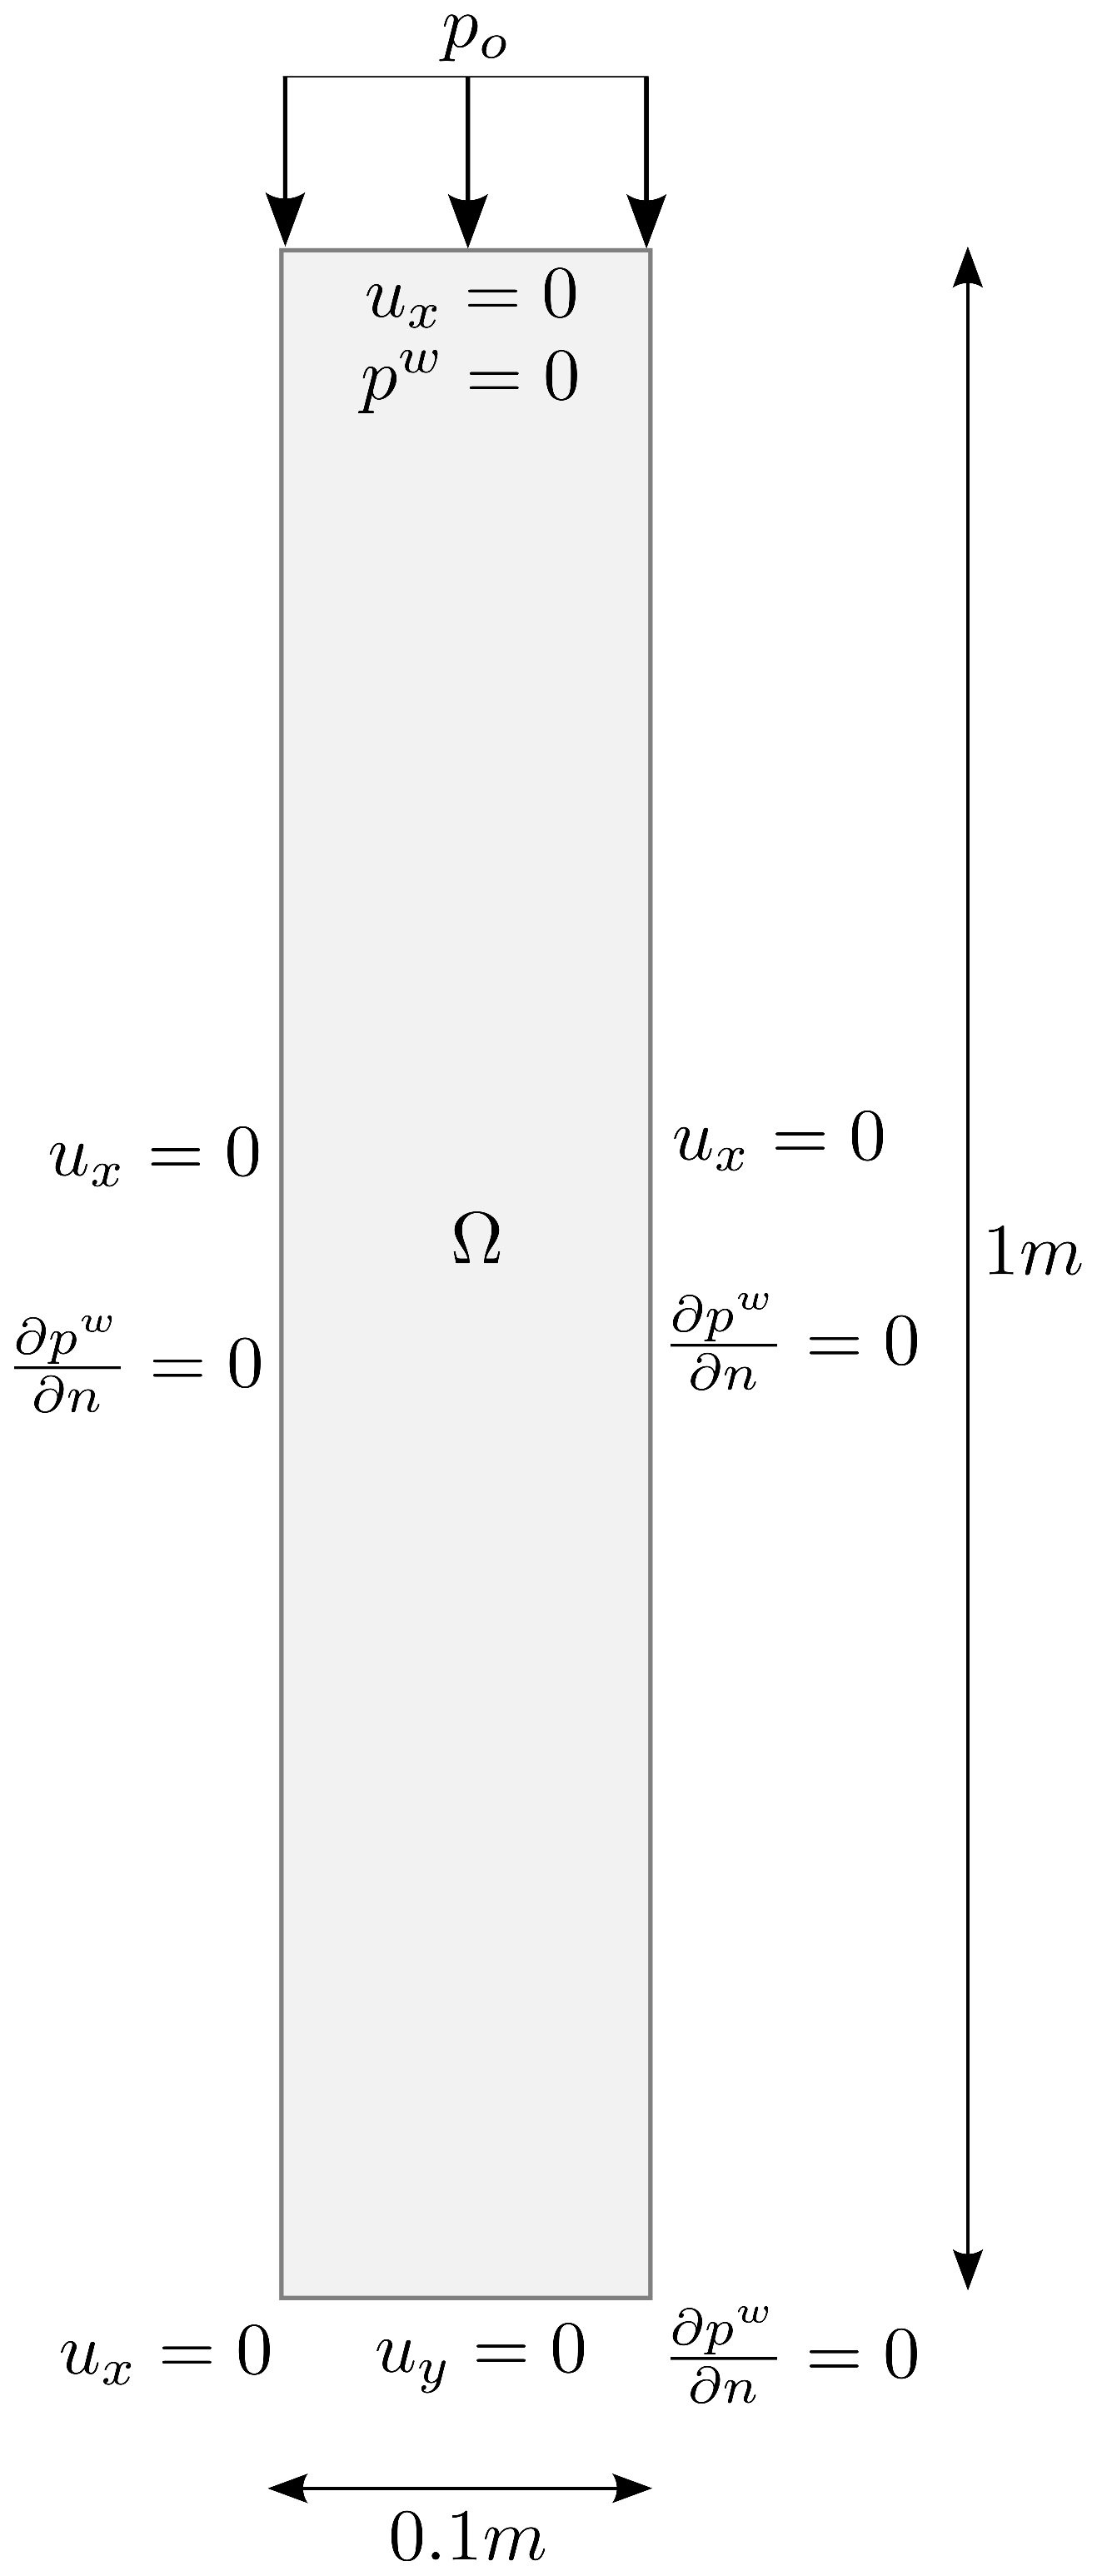
\includegraphics[height=7cm]{figs/Benchmark2}
  \end{center}
  \end{wrapfigure}
  \begin{align*}
    E &= \SI{30}{\kilo\pascal} \\
    \nu &= 0.2 \\
    k &= \SI{98.1}{\milli\meter\per\second} \\
    p_0 &= \SI{1}{\kilo\pascal}
  \end{align*}
  \hspace{6cm}Similar type of analytical solution.
\end{frame}

\begin{frame}
  \frametitle{1D consolidation}

  \begin{center}
    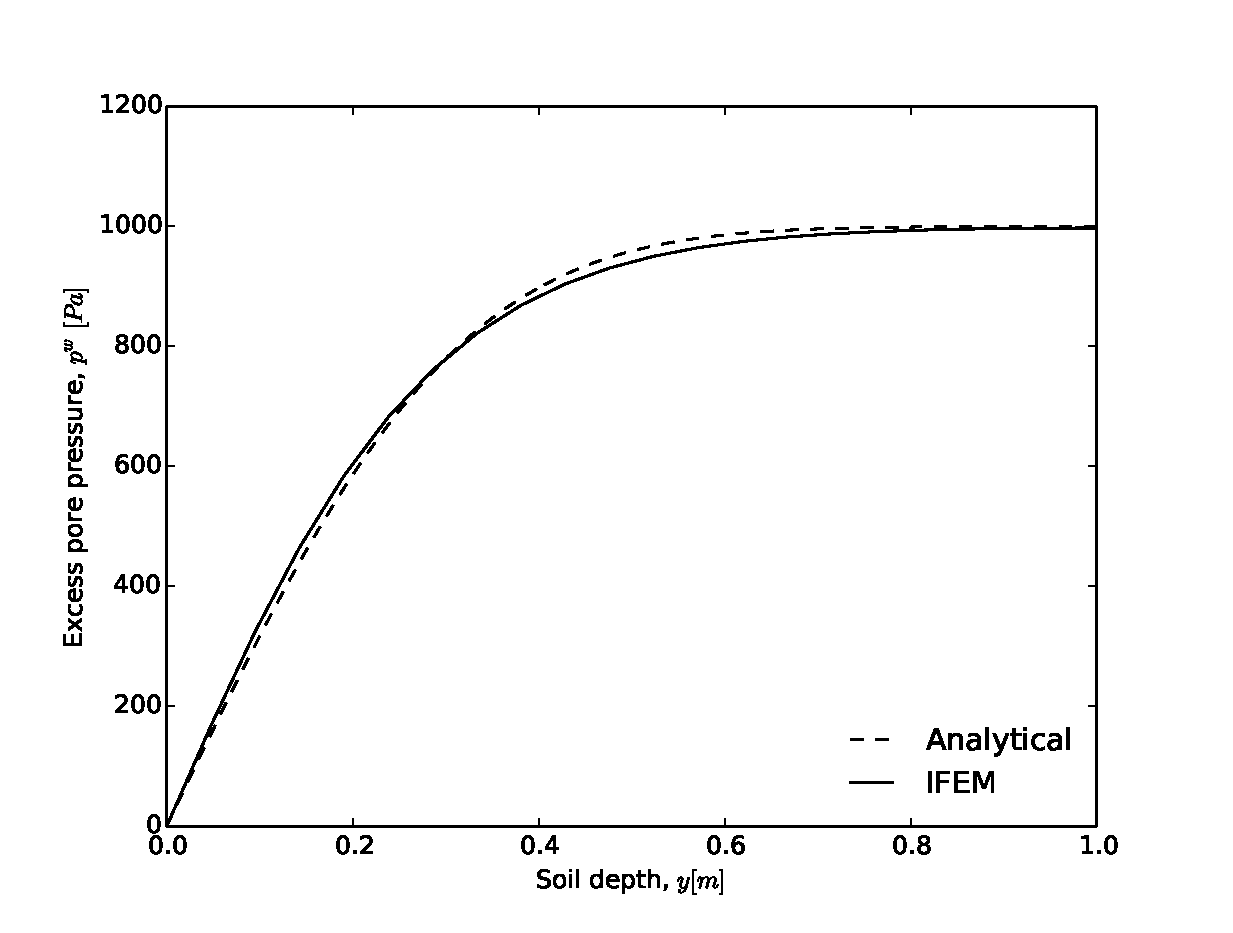
\includegraphics[height=7cm]{figs/OGS1D_Anasol_v_IFEM}
  \end{center}
\end{frame}

\begin{frame}
  \frametitle{2D consolidation}

  Same physical quantities as in the previous problem.
  \begin{center}
    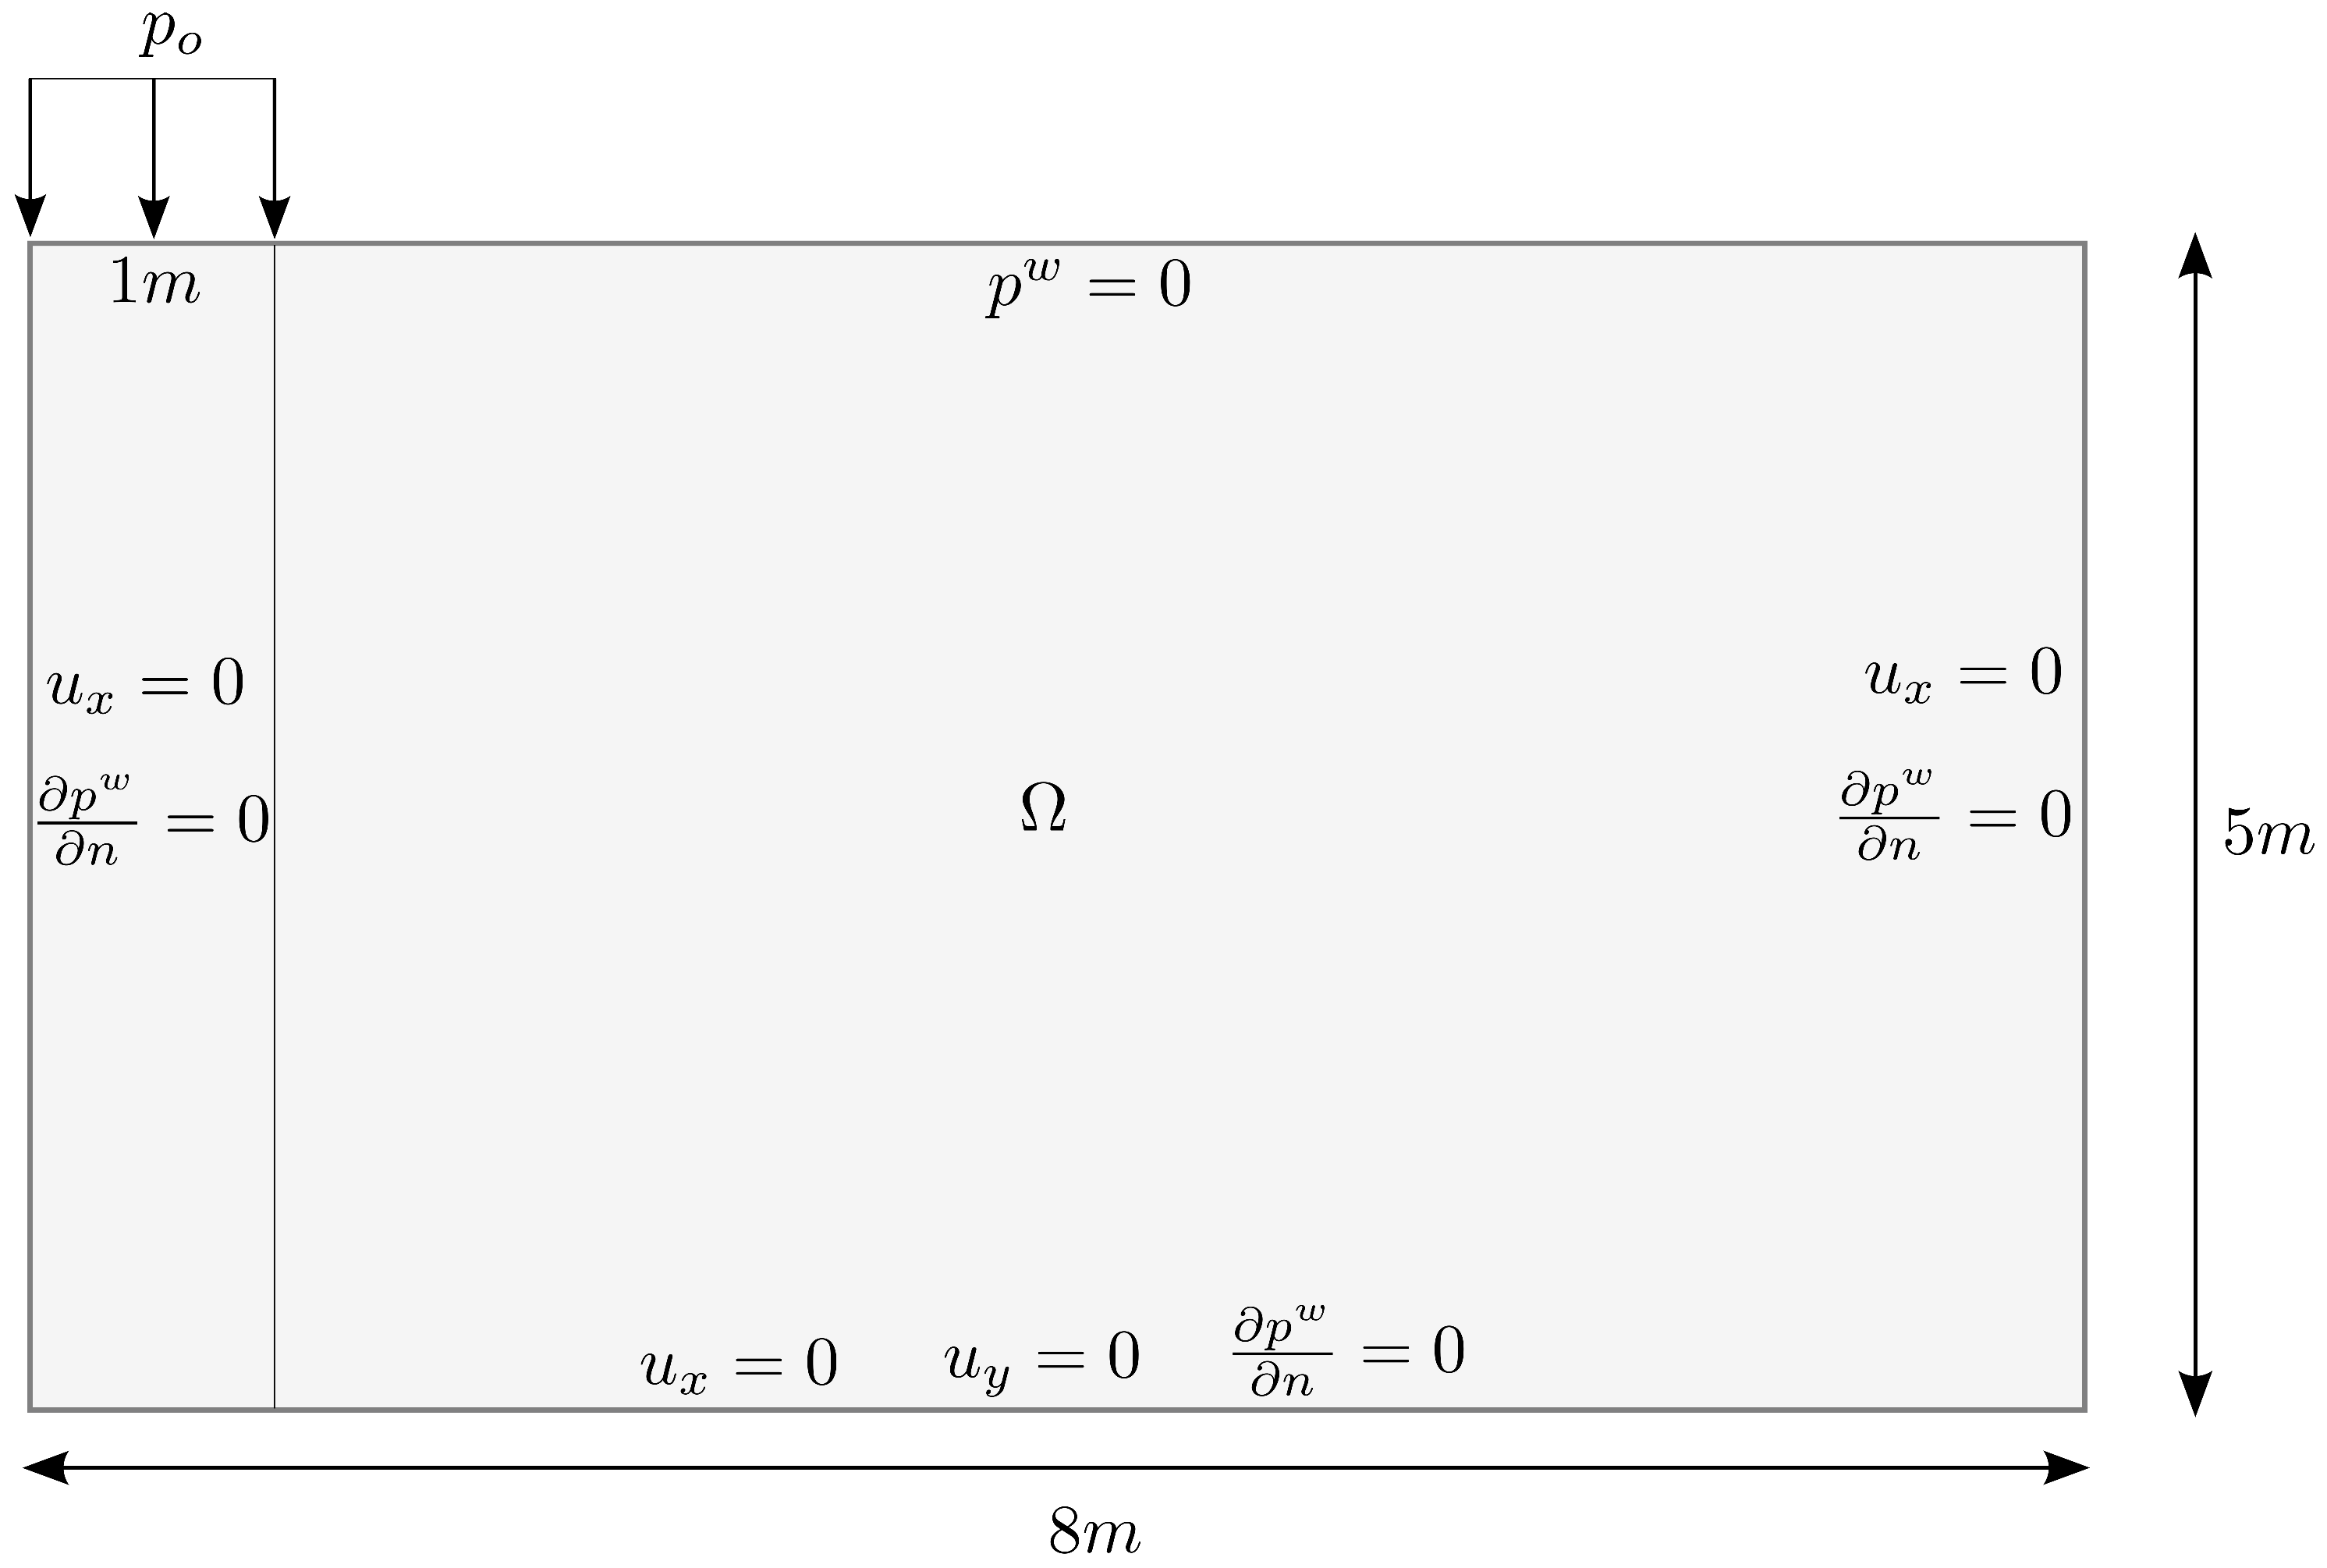
\includegraphics[height=6cm]{figs/Benchmark3}
  \end{center}
\end{frame}

\begin{frame}
  \frametitle{2D consolidation}

  Multipatch model with $C^0$-continuity across the boundary.
  \begin{center}
    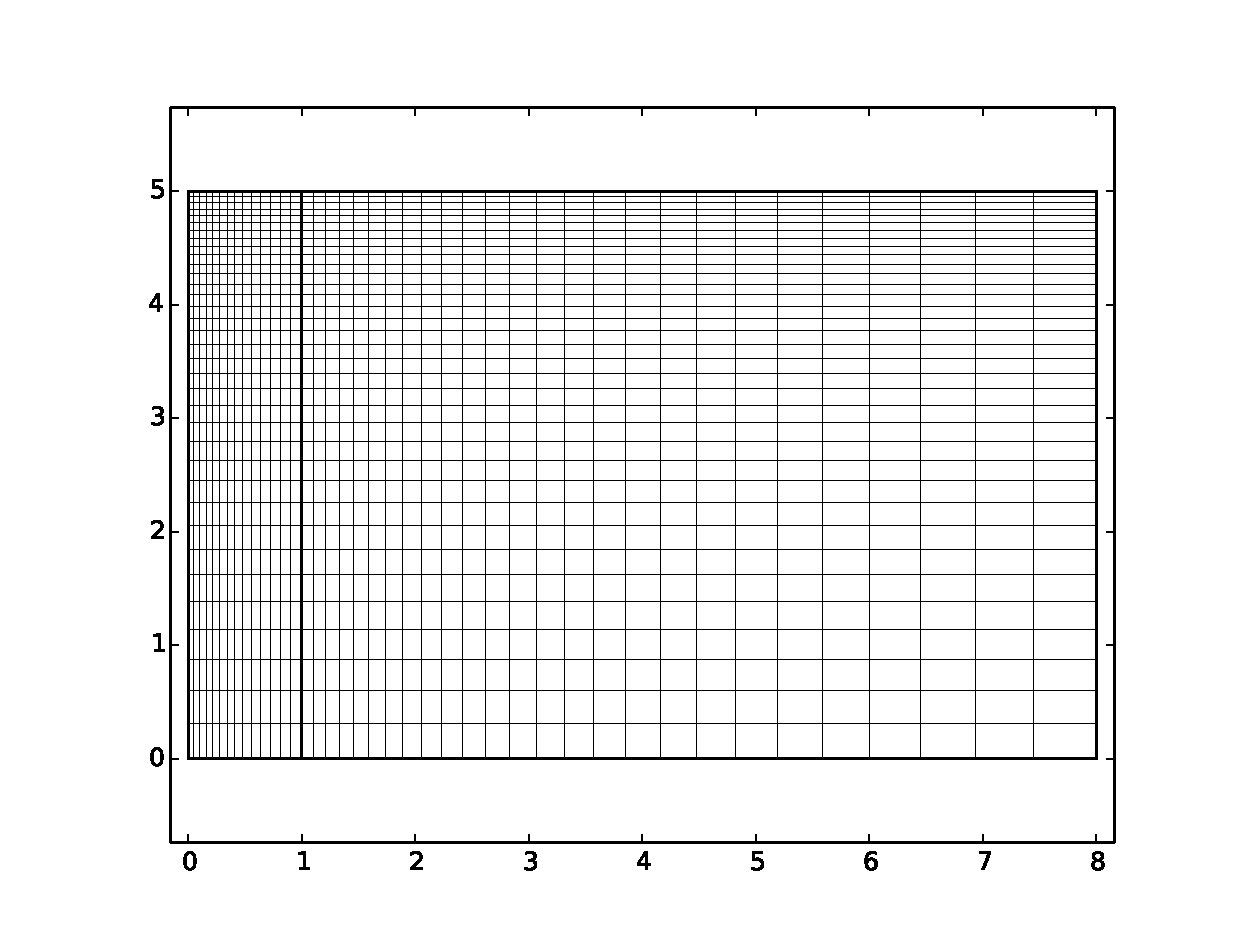
\includegraphics[height=6cm]{figs/OGSBenchmark2Dgraded}
  \end{center}
\end{frame}

\begin{frame}
  \frametitle{2D consolidation}

  Pressure distribution at $t = \SI{4}{\second}$.
  \begin{center}
    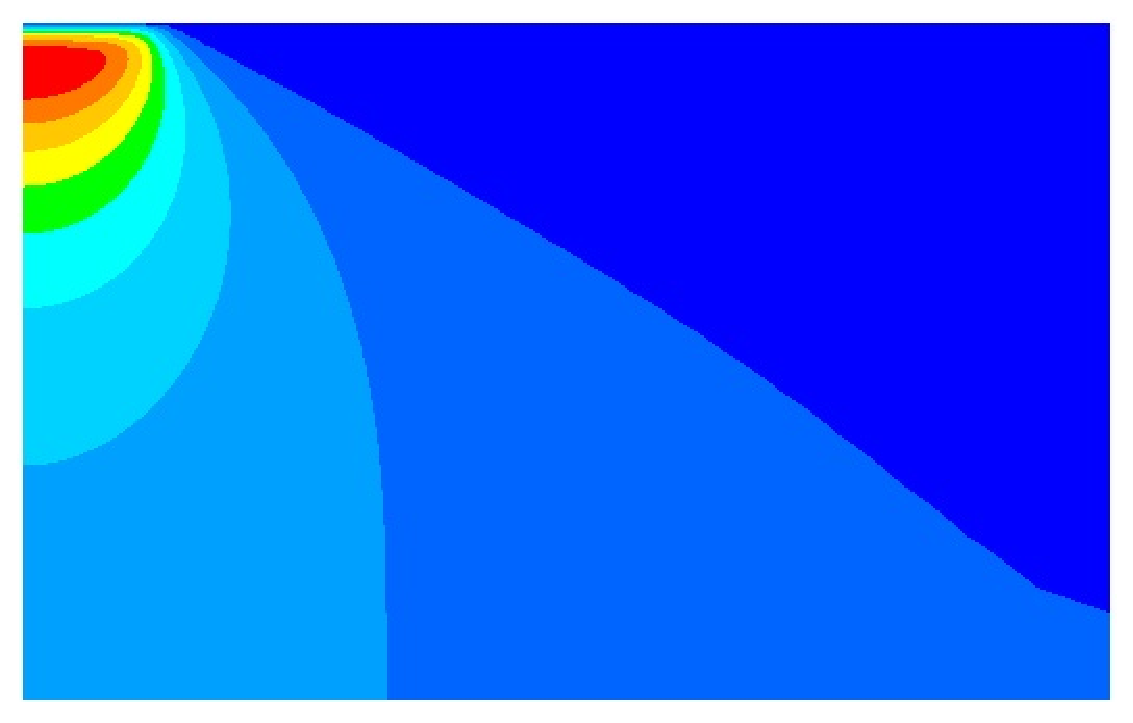
\includegraphics[height=6cm]{figs/OGS2DExcessPorePrDist}
  \end{center}
\end{frame}

\begin{frame}
  \frametitle{2D consolidation}

  Pressure distribution at $t = \SI{4}{\second}$, left edge.
  \begin{center}
    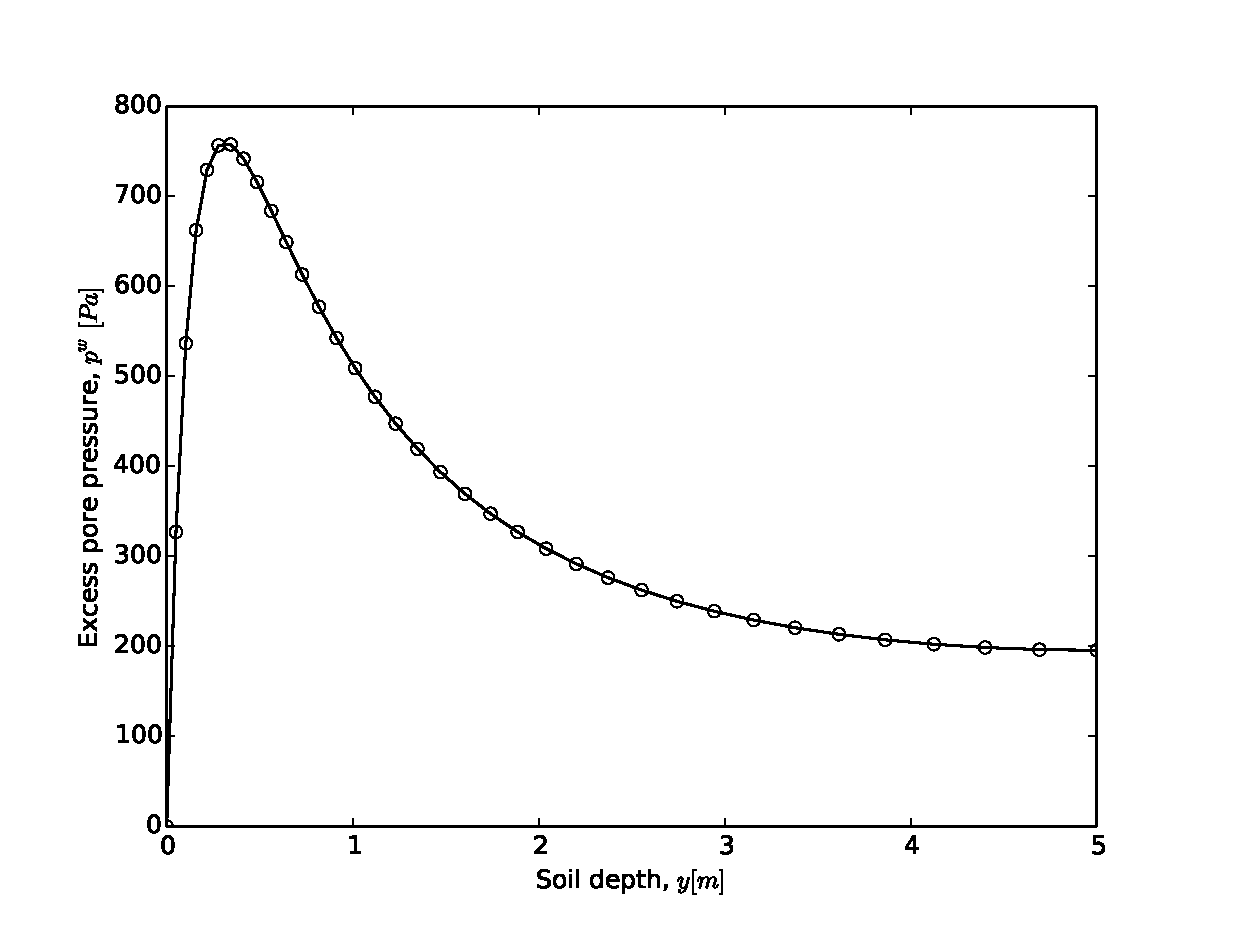
\includegraphics[height=6cm]{figs/OGS2DExcessPorePrProf}
  \end{center}
\end{frame}

\begin{frame}
  \frametitle{Pressure oscillations}

  Case due to Joachim Berdal Haga.
  \begin{center}
    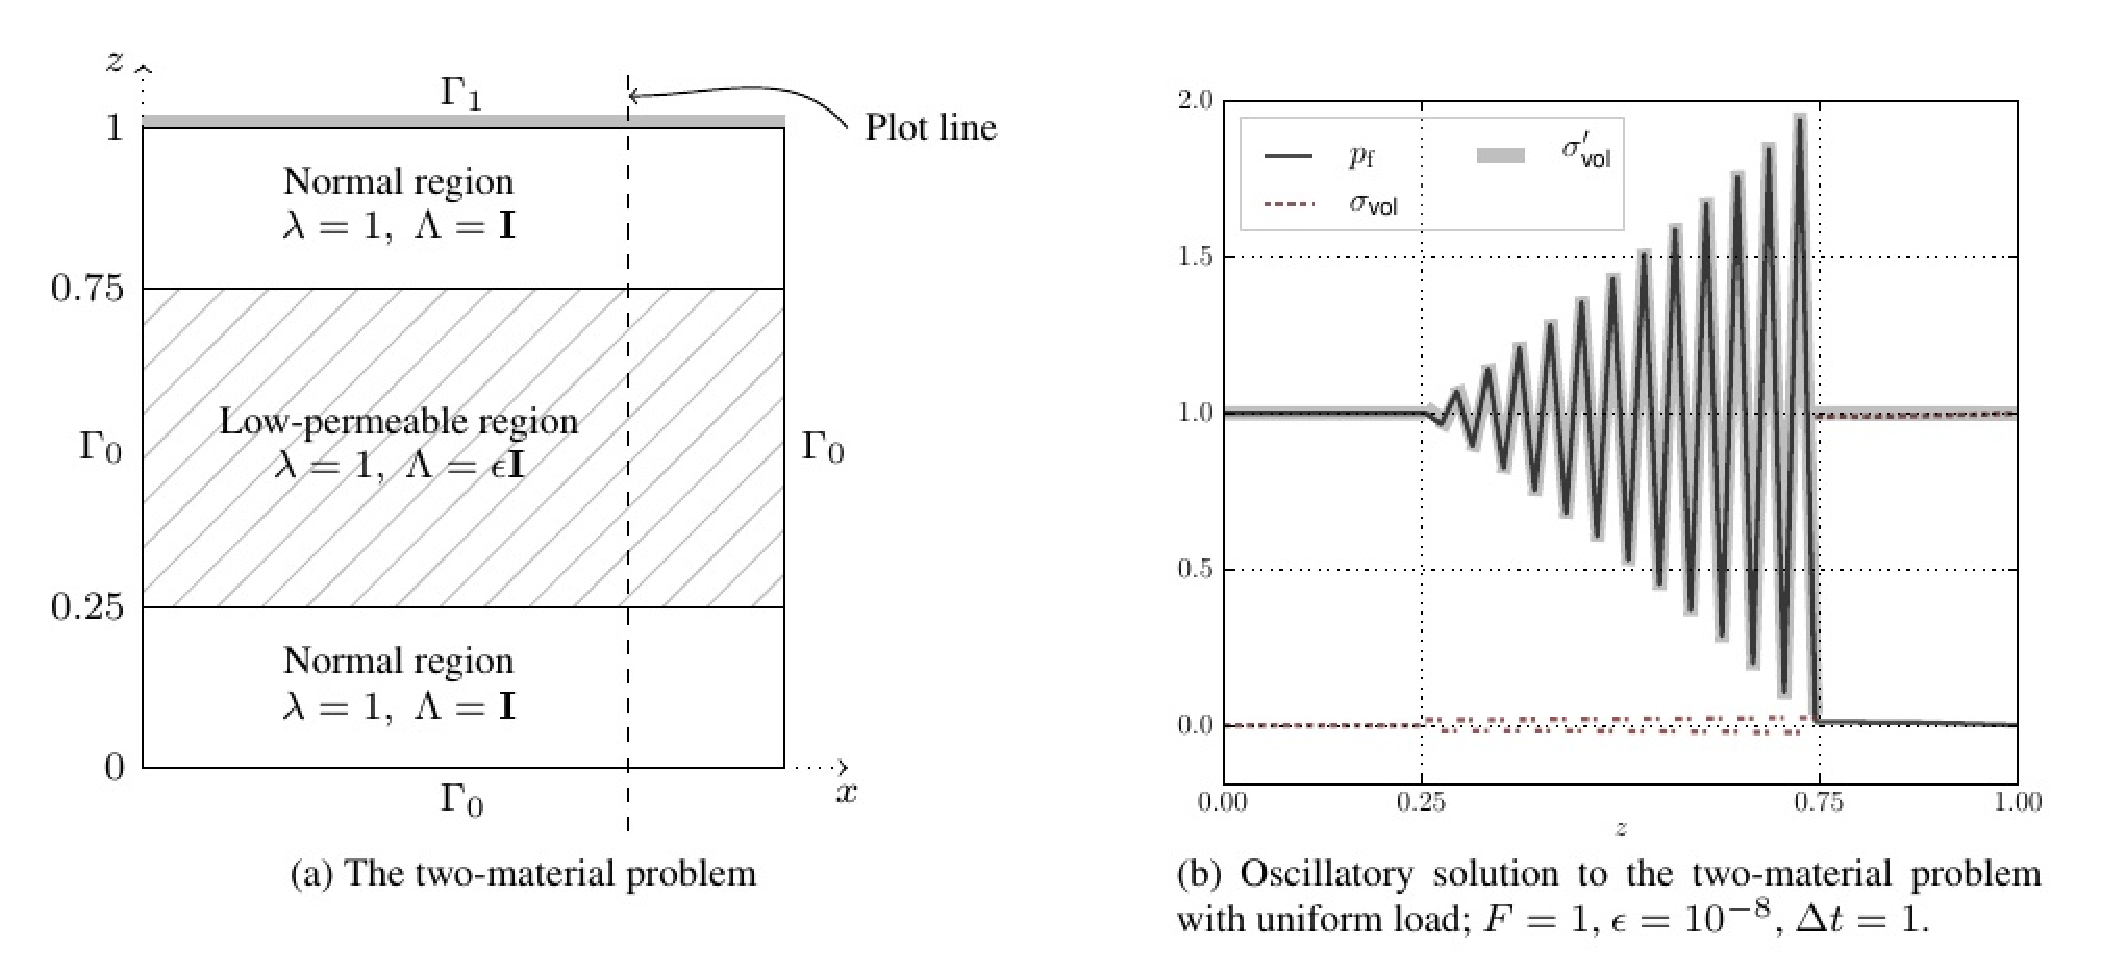
\includegraphics[width=12cm]{figs/PressureOscillationsProblem}
  \end{center}
\end{frame}

\begin{frame}
  \frametitle{Pressure oscillations}

  $C^0$-discontinuous model at, the boundary layers.
  \begin{center}
    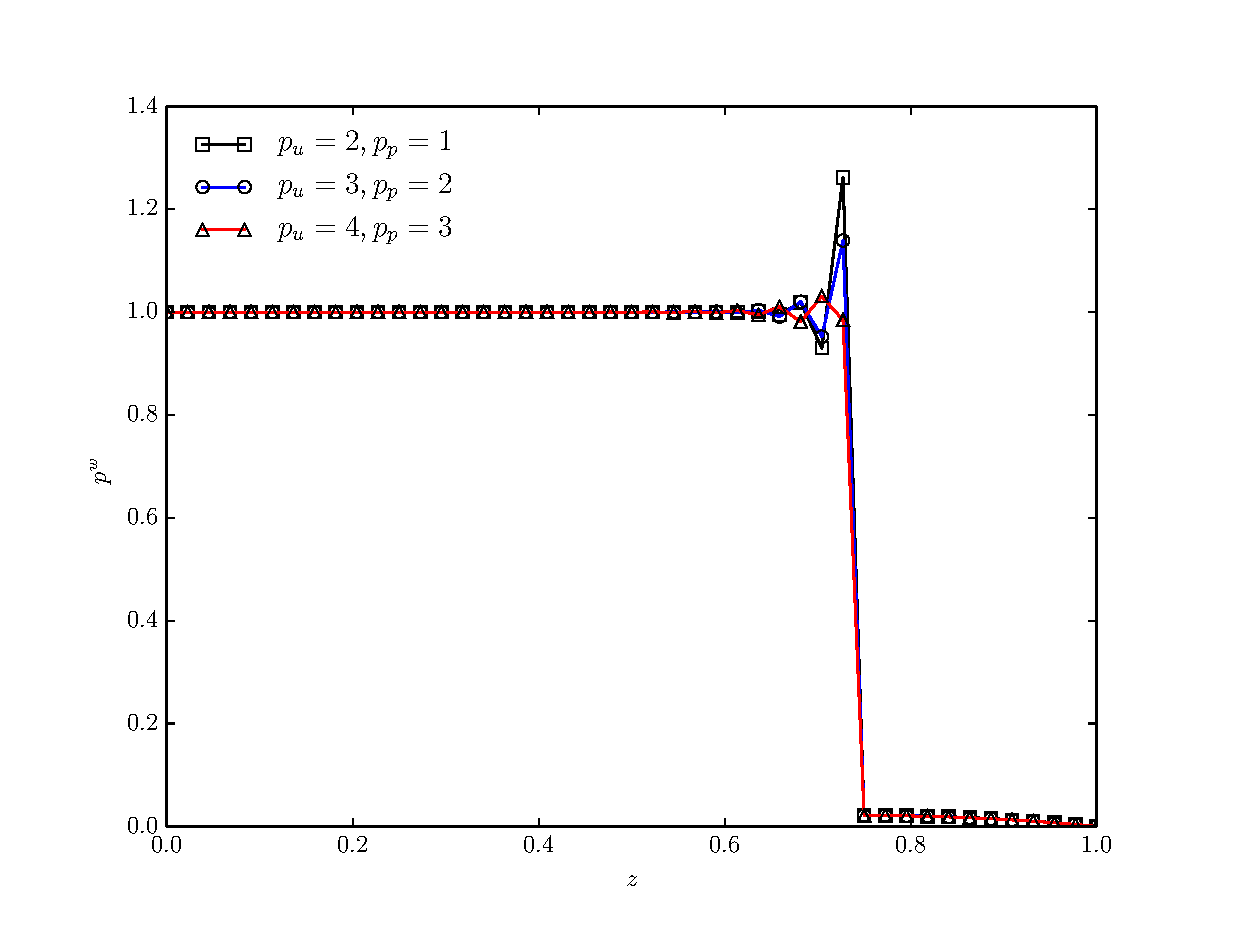
\includegraphics[height=6cm]{figs/LowPermLayer_pw-z_plot7}
  \end{center}
\end{frame}

\begin{frame}
  \frametitle{Pressure oscillations}

  $C^0$-discontinuous model at the boundary layers.
  \begin{center}
    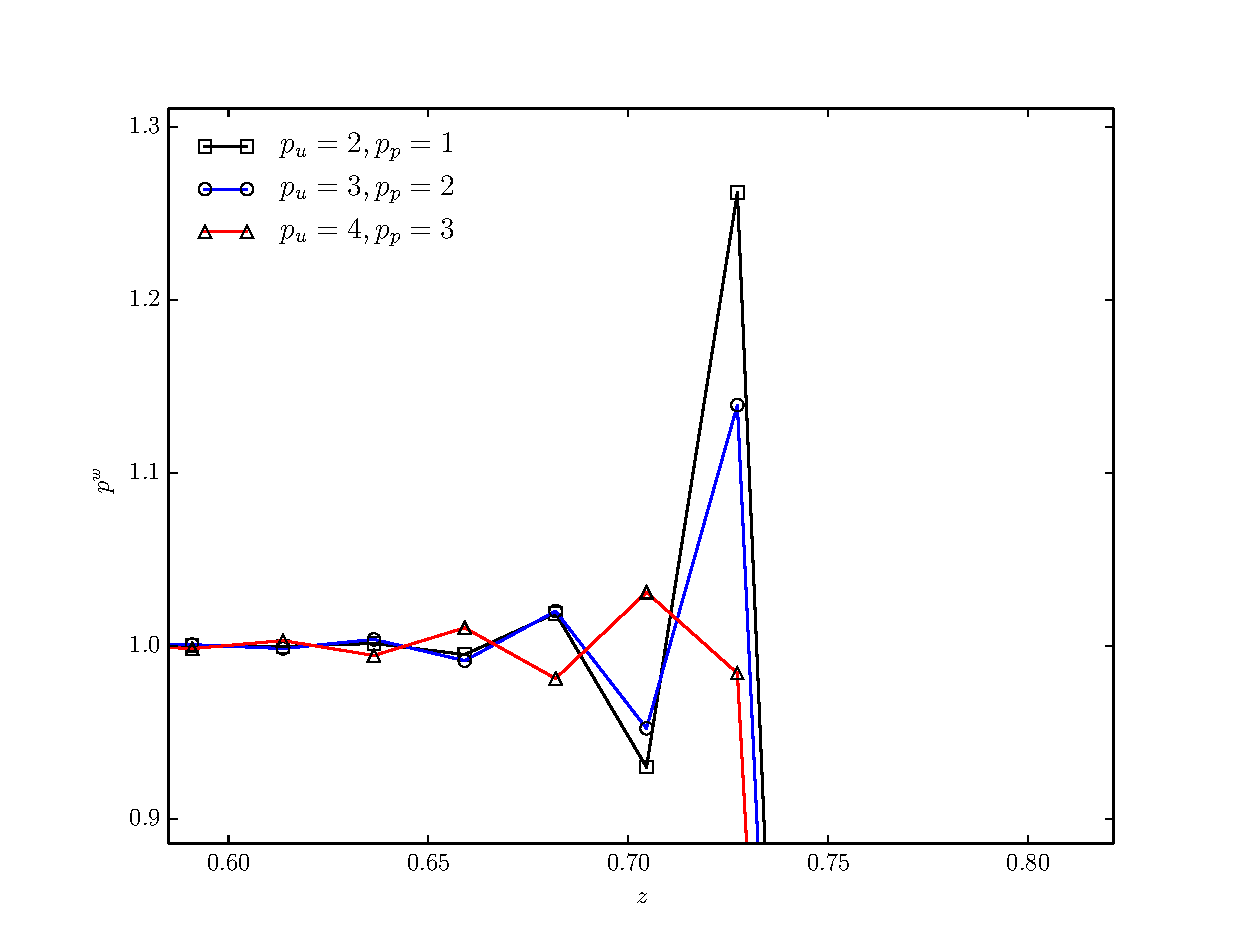
\includegraphics[height=6cm]{figs/LowPermLayer_pw-z_plot6}
  \end{center}
\end{frame}

\begin{frame}
  \frametitle{Pressure oscillations}

  $C^{-1}$-discontinuous model at the boundary layers.
  \begin{center}
    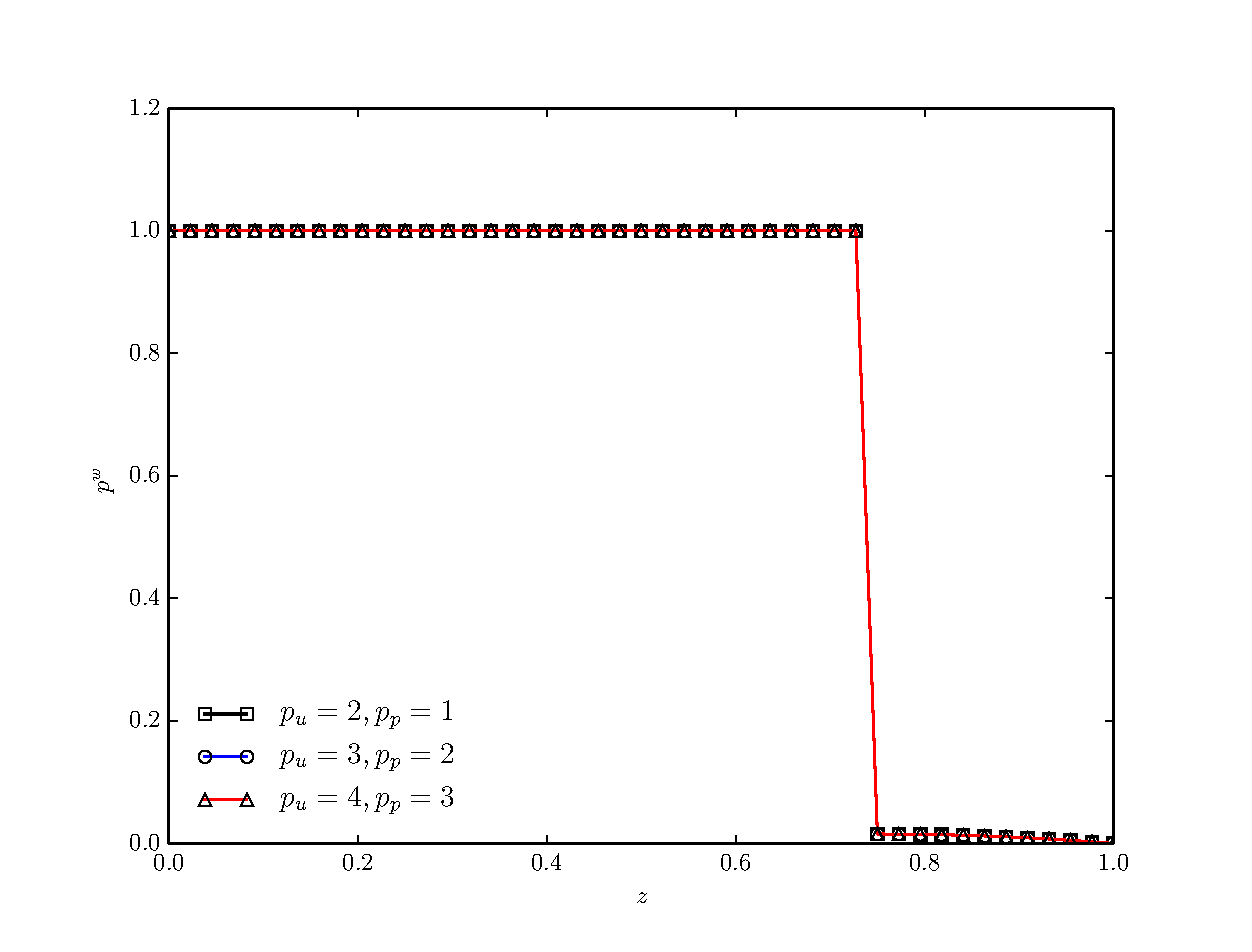
\includegraphics[height=6cm]{figs/LowPermLayer_pw-z_plot8}
  \end{center}
\end{frame}

\begin{frame}
  \frametitle{Conclusions and Future work}

  Conclusions
  \begin{itemize}
  \item Mixed-order methods can alleviate pressure oscillations.
  \item \ldots so can knot insertion.
  \end{itemize}

  Expected future work
  \begin{itemize}
  \item 3D. Should in principle already work. (Thanks, IFEM.)
  \item Adaptivity using LR B-splines. Should in principle also already work for
    single-patch models.
  \item Div-compatible spaces.
  \item Fracture mechanics.
  \end{itemize}
\end{frame}

\end{document}
